Los resultados obtenidos en cada uno de los pasos de este trabajo se detallan en
este capítulo, comenzando por el motor obtenido en la primera iteración de
optimización con el algoritmo genético junto con el modelo geométrico 3D
generado.
%
Luego se muestran los resultados de las flujometrías realizadas a partir del
modelo de CAD, incluyendo las mallas obtenidas para algunos casos seleccionados
y el resultado detallado de algunas de las flujometrías, finalizando con el mapa
de $C_{D}$ obtenido, tanto para el puerto de admisión como para
el puerto de escape.

Por último se presentan los resultados de la segunda ronda de optimización con
el algoritmo genético, en la que se utilizó el mapa de $C_{D}$ obtenido en el
paso previo.

\section{Primera Iteración}
%
La primera optimización se realizó partiendo de una población al azar, con los
coeficientes de descarga constantes de 0,7 y 0,75 para el puerto de admisión y
escape respectivamente.
%
El algoritmo genético se ejecutó durante 100 generaciones con una población de
100 individuos y la función objetivo definida en la
sección~\ref{sec:funcion_objetivo} con los pesos, operadores y
parámetros correspondientes indicados en la Tabla~\ref{tab:config_genetico}.

\begin{table}[ht!]
  \centering
  \begin{tabular}{ccc} \toprule
    Parámetro & Valor & Unidad \\ \midrule
    RPMS & $1000\times[1, 2, 3, 4, 5, 6, 7, 8, 9]$ & \\
    Pesos de función objetivo & $(1, 1, 1, 6, 8, 9, 8, 7, 7)$ & \\
    Diámetro mínimo & 0,05 & m \\
    Diámetro máximo & 0,1 & m \\
    Longitud mínima de tubo & 0,5 & m \\
    Longitud máxima de tubo & 2 & m \\
    Ángulo mínimo & 0 & grados \\
    Ángulo máximo & 90 & grados \\
    Separación angular máxima & 70 & grados \\
    Tamaño de población & 100 & - \\
    Tamaño de torneo & 10 & - \\
    Probabilidad de cruza & 0,9 & - \\
    Probabilidad de mutación & 0,5 & - \\
    Cantidad de generaciones & 20 & - \\
    Tamaño de \emph{SALÓN DE LA FAMA} & 1 & - \\ \bottomrule
    \end{tabular}
  \caption{Configuración utilizada.}\label{tab:config_genetico}
\end{table}

% Nota: terminar de agregar la figura
% Para ICESym se utilizaron dos ciclos de simulación, por considerarse que es
% suficientemente preciso para esta primer aproximación.
%
% En la Figura XX se puede ver que a partir de la segunda iteración se obtienen
% buenos resultados, esto se debe a que los datos de partida para la segunda
% iteración, son los resultados de la primer iteración.
%

En la gráfica de evolución se observa que se obtuvo rápidamente un individuo con
un puntaje relativamente alto en las primeras iteraciones.
%
El resultado final tiene una aptitud 1.5 veces la aptitud media de la población
de la última generación, siendo los parámetros que definen este candidato los
listados en la Tabla~\ref{tab:resultado_primer_it} y se ilustran en la
Figura~\ref{fig:primer_op}.
%
Este motor tiene un rendimiento volumétrico máximo de $\eta_{v} \simeq 0.83$
para 2500 RPM y si bien la función objetivo favorece curvas suaves, se ven dos
picos de rendimiento en la curva, siendo el segundo con $\eta_{v} \simeq 0.79$ a
7500 RPM.

A modo de comparación, en la misma tabla se presentan las características
geométricas obtenida en trabajos anteriores~\parencite{mrcvc:sim_computacional}.

\begin{figure}[ht]
  \centering
  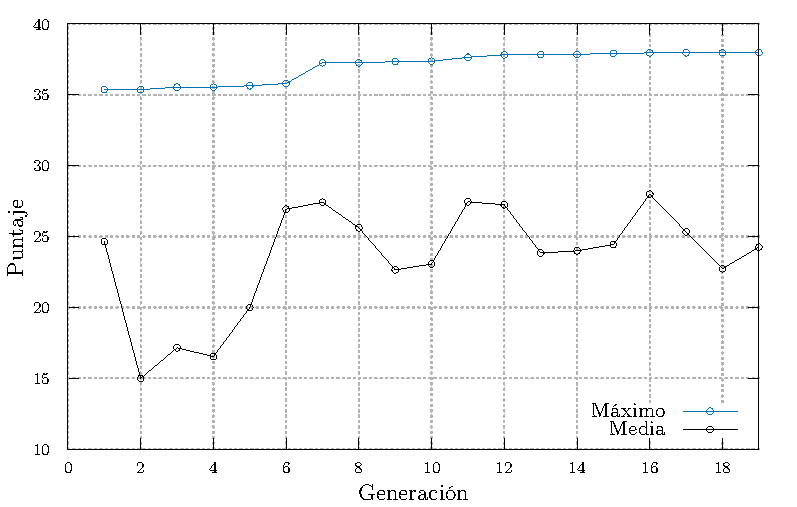
\includegraphics[width=.8\textwidth]{gnuplot/genetico.pdf}
  \caption{Evolución de la población} \label{fig:ev_primer_op}
\end{figure}%
\begin{figure}[ht]
  \centering
  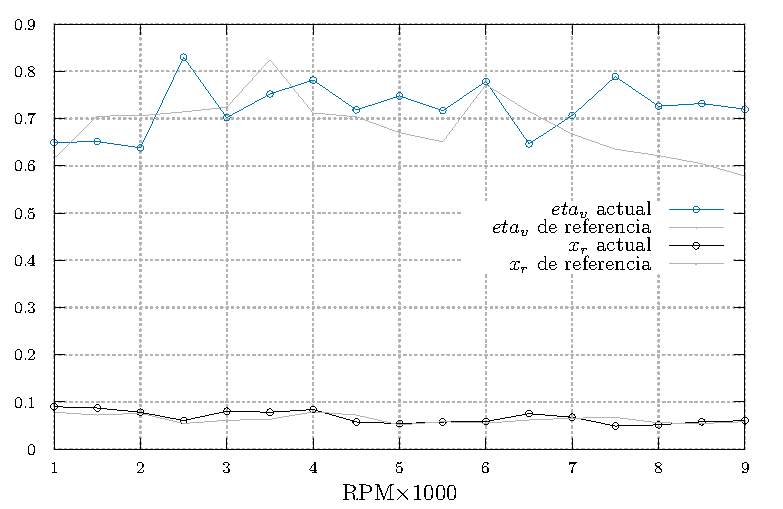
\includegraphics[width=.8\textwidth]{gnuplot/primer-rendimiento.pdf}
  \caption{Rendimiento volumétrico y fracción de gases residuales del motor seleccionado} \label{fig:primer_op}
\end{figure}

\begin{table}
  \centering
  \begin{tabular}{ccccc} \toprule
    Parámetro & Inicial & Actual & Inicial & Actual \\
    Longitud del tubo [mm] & 1300 & 519 & 800 & 976 \\
    Diámetro del tubo [mm] & 70 & 97 & 50 & 81 \\
    Ángulo de apertura del puerto [$\circ$] & 519.93 & 1.12 & 396.87 & 85.15 \\
    Ángulo de cierre del puerto [$\circ$] & 175.76 & 70.15 & 587.06 & 11.13 \\ \bottomrule
  \end{tabular}
  \caption{Datos geométricos del mejor candidato}\label{tab:resultado_primer_it}
\end{table}


En la Figura~\ref{fig:PoTi_primer_op} se muestran las curvas de potencia y
torque del motor.
%
Como es de esperarse se ve que ambas copian la curva de rendimiento volumétrico,
con una potencia al freno máxima de 142 CV a 6500 RPM y un torque máximo de 194
N.m a\ 4000 RPM.

\begin{figure}[ht]
  \centering
  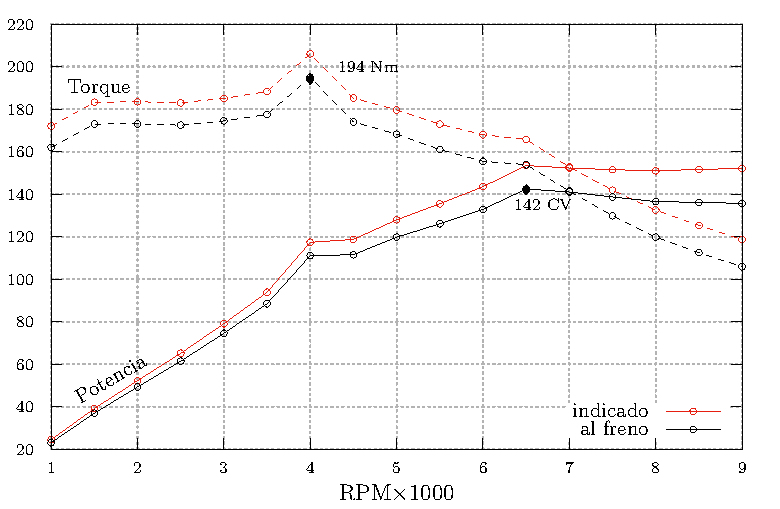
\includegraphics[width=\textwidth]{gnuplot/primer-potencia.pdf}
  \caption{Torque y Potencia de Primera Iteración} \label{fig:PoTi_primer_op}
\end{figure}


\section{Modelo de CAD}
%
A partir de los resultados obtenidos se realizó un modelo de CAD de los puertos
que se ilustra en las Figuras~\ref{fig:motor_cad1} y~\ref{fig:motor_cad2}.
%
Se representó solamente la mitad superior del motor que contiene ambos puertos
de admisión y escape, este modelo es paramétrico y permite rotar los componentes
del motor para obtener distintas posiciones del conjunto y así poder generar la
geometría a evaluar con las flujometrías.

% Algunos redondearon las aristas internas incluyendo las paletas y las puntas del rotor para favorecer el proceso de mallado, ya que los bordes agudos pueden ser problmeáticos para el mallador \emph{snappyHexMesh}.

\begin{figure}[ht]
  \centering
    \begin{subfigure}{0.4\textwidth}
        \centering
        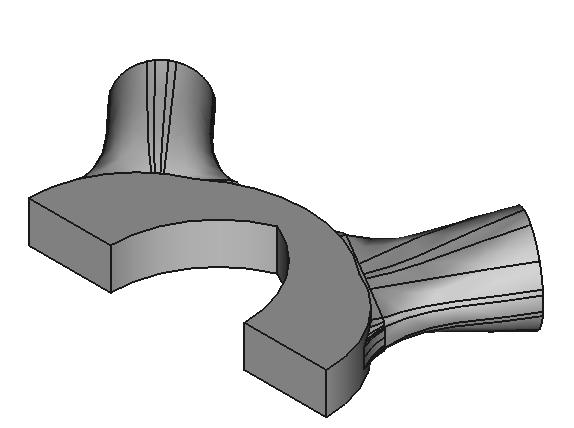
\includegraphics[width=\textwidth]{CAD/motor_cad1.png}
    \end{subfigure}
    \hfill
    \begin{subfigure}{0.4\textwidth}
        \centering
        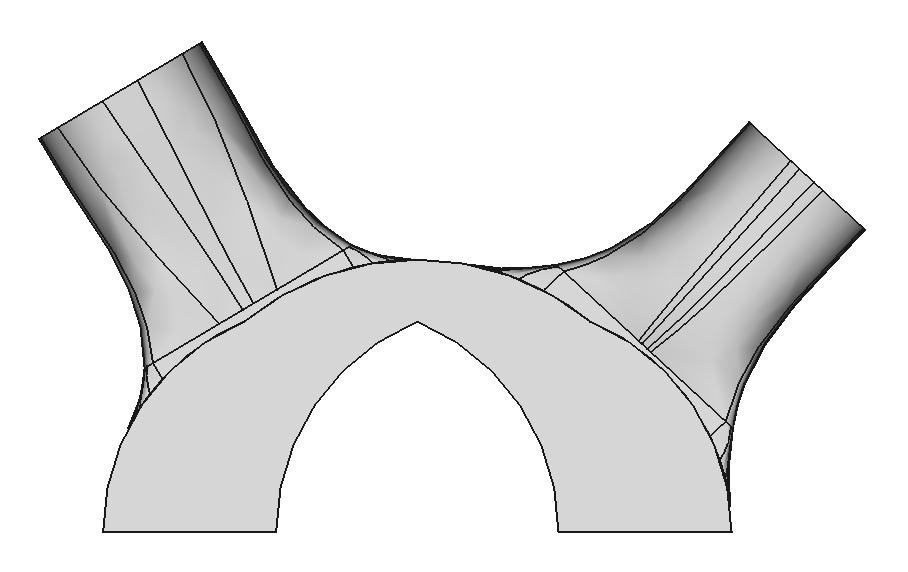
\includegraphics[width=\textwidth]{CAD/motor_cad2.png}
    \end{subfigure}
  \caption{CAD Primera iteración}\label{fig:motor_cad1}
\end{figure}


\begin{figure}[ht]
  \centering
    \begin{subfigure}{0.8\textwidth}
        \centering
        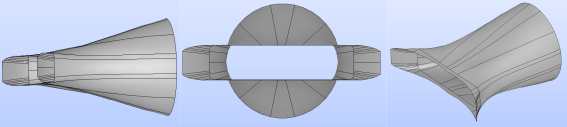
\includegraphics[width=\textwidth]{CAD/vistas_admision.png}
        \caption{Puerto de Admsisión.}
    \end{subfigure}
    \begin{subfigure}{0.8\textwidth}
        \centering
        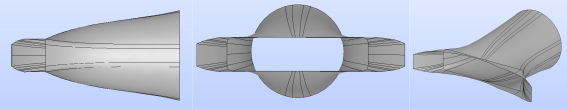
\includegraphics[width=\textwidth]{CAD/vistas_escape.png}
        \caption{Puerto de Escape.}
    \end{subfigure}
  \caption{CAD Primera iteración (vistas fuera de escala).}\label{fig:motor_cad2}
\end{figure}

La altura del puerto del lado de la cámara se mantuvo en dos tercios de la
altura de la cámara $h_{p} = \frac{2}{3}h_{c}$, manteniendo el eje central de cada
puerto de forma que intersecte el centro del motor con el propósito de eliminar
una variable de la geometría a modelar.
%
El foco de esta etapa de optimización es el diámetro del puerto y el reglaje.
%

%%%%%%%%%%%%%%%%%%%%%%%%%%%%%%%%%%%%%%%%%%%%%%%%%%%%%%%%%%%%%%%%%%%%%%%%%%%%%%%
